% https://tex.stackexchange.com/a/763399/322482
\documentclass[tikz,border=1cm]{standalone}
\usepackage{fourier}
\usepackage{amsmath}
\DeclareMathOperator{\arr}{arr}
\DeclareMathOperator{\first}{first}

\usepackage{fdsymbol}
\usetikzlibrary{positioning,fit}
\begin{document}
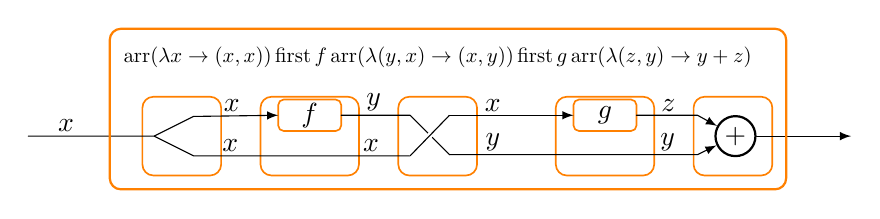
\begin{tikzpicture}[
    line join=round,line cap=round,
    mybox/.style 2 args={rounded corners,inner sep=0pt,outer sep=0pt,minimum width=#1cm,minimum height=#2cm,draw=orange,semithick},
]
\node[mybox={1}{1}] (B3) {};
\node[mybox={1.25}{1},left = .5cm of B3] (B2) {};
\node[mybox={1}{1},left = .5cm of B2] (B1) {};
\node[mybox={1.25}{1},right = 1cm of B3] (B4) {};
\node[mybox={1}{1},right = .5cm of B4] (B5) {};

\coordinate (A) at ([xshift=-1.45cm]B1.west);

\node[mybox={.8}{.4},anchor=north,rounded corners=2pt] (f) at ([yshift=-1pt]B2.north) {$f$};
\node[mybox={.8}{.4},anchor=north,rounded corners=2pt] (g) at ([yshift=-1pt]B4.north) {$g$};


\draw[-latex] (A) -- node[above=-2pt,pos=.3] {$x$} ++(1.6,0) coordinate (tmp1) -- ++ (.5,.25) -- node[above=-2pt,pos=.45] {$x$}(f.west);

\draw (tmp1) -- ++ (.5,-.25) -- node[above=-2pt,pos=.17] {$x$} node[above=-2pt,pos=.82] {$x$}  ++(2.75,0) coordinate (tmp2);

\coordinate (tmp3) at (f.east-|tmp2);

\draw (f.east) -- node[above=-2pt,pos=.47] {$y$} (tmp3) -- ++(.5,-.5) coordinate (tmp4) ++ (0,.5) coordinate (tmp5);

\draw[white,double=black,thick,double distance=.4pt,line cap=butt] (tmp2) -- (tmp5);

\draw[-latex] (tmp5) -- node[above=-2pt,pos=.35] {$x$} (g.west);

\node[circle,draw,thick,anchor=east,inner sep=1.5pt] (plus) at ([xshift=-.2cm]B5.east) {$+$};

\draw[-latex] (tmp4) -- node[above=-2pt,pos=.175] {$y$} node[above=-2pt,pos=.88] {$y$} ++(3.15,0) coordinate (tmp6) -- (plus);

\coordinate (tmp7) at (g.east-|tmp6);
\draw[-latex] (g.east) -- node[above=-2pt,pos=.525] {$z$}  (tmp7) -- (plus);
\draw[-latex] (plus.east) -- ++(1.2,0);

\node[mybox={10}{.5},draw=none,scale=.75] (txt) at (0,1) {$\arr (\lambda x \to (x,x)) \ggg \first f \ggg \arr (\lambda(y,x) \to (x,y)) \ggg \first g \ggg \arr (\lambda(z,y) \to y+z)$};

\node[fit=(txt)(B1)(B5),inner sep=5pt,draw=orange,thick,rounded corners] {};

\end{tikzpicture}

\end{document}